\subsection{VON}
\label{chap:related:von}
\ac{von} ist in seinen Grundzügen stark unterschiedlich zu den bisher vorgestellten Umsetzungen. \ac{von} nutzt das \ac{p2p}-Netzwerk nicht nur als Kommunikationsmedium, sondern auch dessen Aufbau als Verteilungsstruktur des Publish/Subscribe-Systems \cite{Hu2006VON}. VON zielt auf die Verteilungsoptimierung von Events zur Positonsänderun, muss allerdings über Applikationswissen verfügen: Die Position des Spielers. \ac{vast} \cite{Backhaus2007Voronoibased} greift das Konzept von \ac{von} auf und testet eine Implementierung auf OpenSIM \cite{Baumgart2007OverSim}.

\begin{figure}[htbp]
\centering
\resizebox{\textwidth}{!}{%
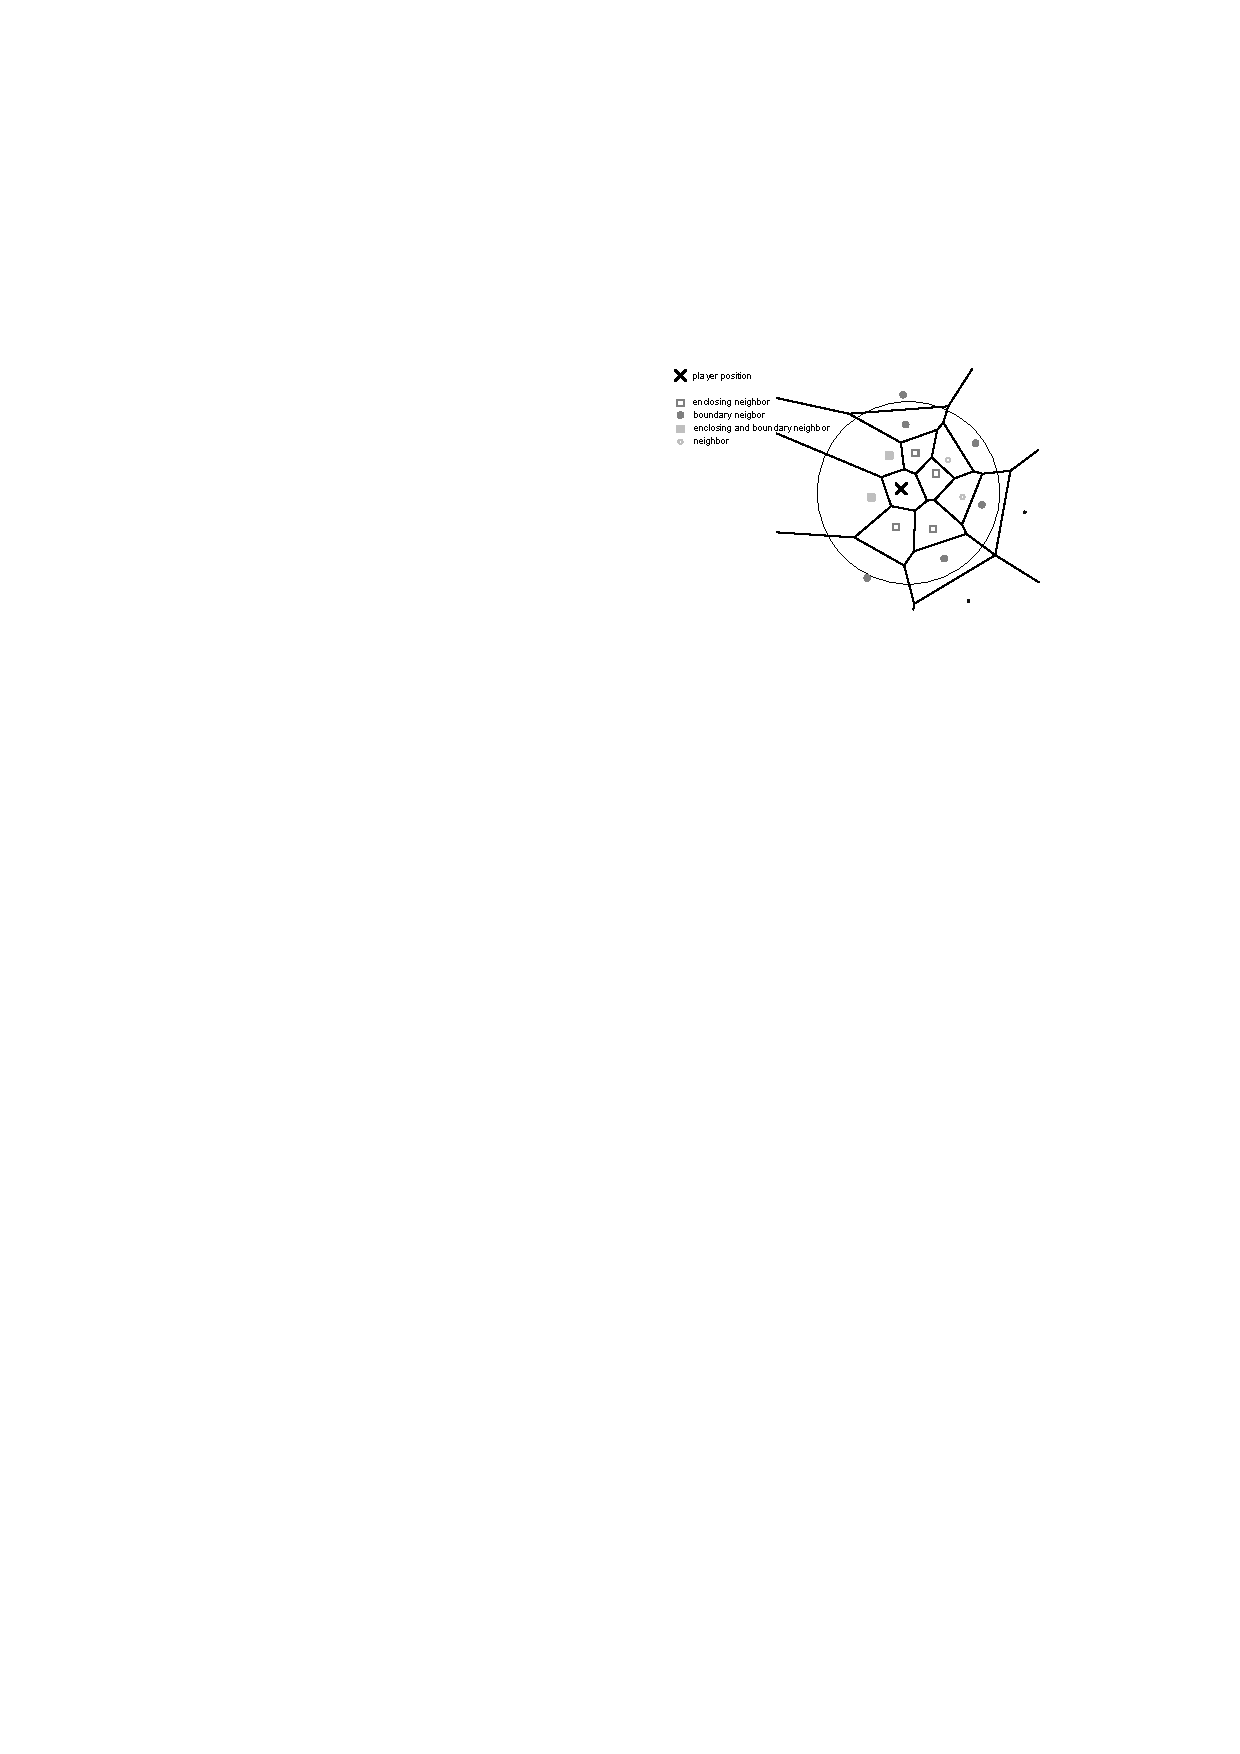
\includegraphics{grafics/voronoi_von_backhaus.pdf}}
\caption{Struktur eines VON-Netzwerkes (aus \cite{Backhaus2007Voronoibased})}
\label{fig:von}
\end{figure}

\Fref{fig:von} zeigt einen Aufbau eines VON-Netzwerks. Die Spielwelt wird anhand der Position der einzelnen Knoten in Voronoi-Diagramme unterteilt. Jeder Knoten hat damit einen eigenen Bereich und hält Verbindungen zu seinen Nachbarn und kennt angrenzende Nachbarn im Bereich seiner \ac{aoi}. ``enclosing neighbors'' sind angrenzende Nachbarn, deren gesamter zugehöriger Bereich innerhalb der \ac{aoi} des Knotens liegt. ``boundary neighbors'' sind nicht angrenzende Knoten, deren eigener Bereich nicht vollkommen innerhalb der \ac{aoi} liegt.

\textbf{Anmeldungen} im Publish/Subscribe-System sind implizit, denn \textbf{Publikationen}, also Positionsänderungen, werden von einem Knoten an alle direkt angrenzenden Nachbarn (``enclosing neighbor'' in \Fref{fig:von}) gesendet. Damit das System konsistent bleibt, werden dabei auch Informationen über andere Nachbarn ausgetauscht. Mit jeder Positionsänderung verändern sich die Aufteilungen des Voronoi-Diagrammes und damit müssen auch die Nachbarschaften angepasst werden.
